\chapter{Joins}
\label{ch:joins}

\begin{chapterintro}
Spark has four ways to run a join and picks one from a size estimate. When the
estimate is right, the choice is right. The estimate comes from table size, and
a table's size says nothing about how much a filter will shrink it: Iceberg
knows \texttt{dim\_product} is 170~MB but not that a \texttt{category} filter
leaves 4~MB of it, so a join that should have broadcast a 4~MB slice shuffles a
billion rows instead. This chapter
covers the four strategies, how the planner chooses between them, and how to
override it when you know better than the statistics do.
\end{chapterintro}

\Cref{fig:join-strategies} shows the shape each strategy leaves in a plan, and \Cref{fig:broadcast-vs-smj} contrasts the
two ends of the cost range. The
rest of this chapter explains why each shape exists and what it costs; the
identifiers to spot them by are catalogued in \Cref{sec:c-joins}.

\begin{figure}[htbp]
  \centering
  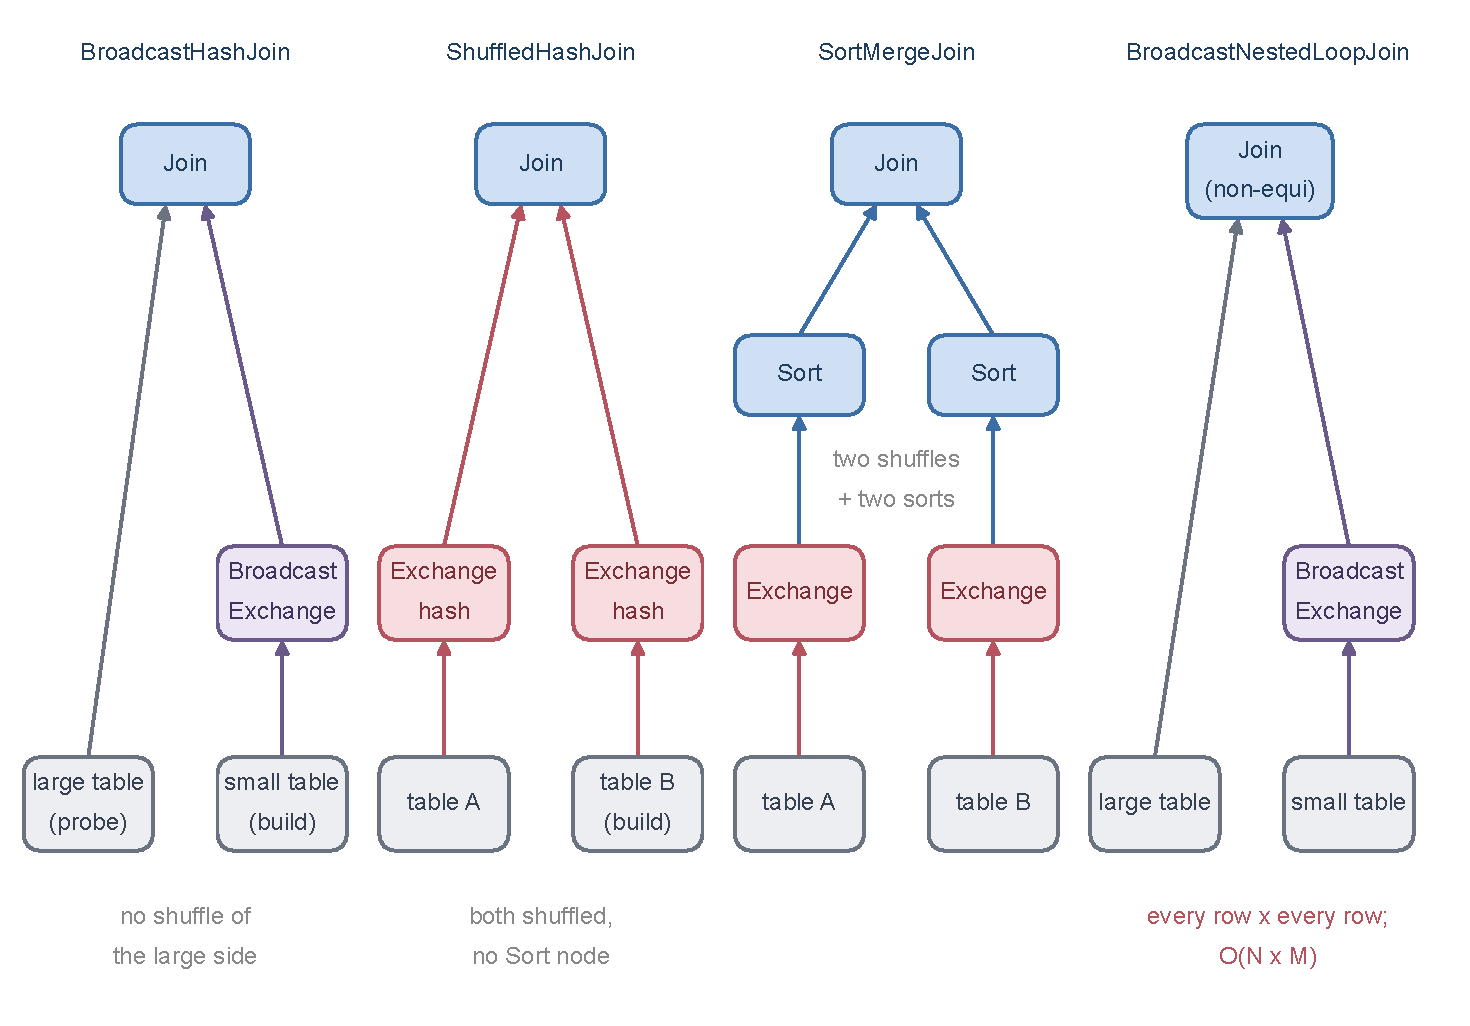
\includegraphics[width=\linewidth]{join-strategies.pdf}
  \caption{The four join strategies as plan shapes. Broadcast hash join shuffles
  nothing on the large side; shuffled hash join shuffles both sides but sorts
  neither; sort-merge join shuffles and sorts both; broadcast nested loop join
  broadcasts one side to evaluate a condition that is not an equality.}
  \label{fig:join-strategies}
\end{figure}

\begin{figure}[htbp]
  \centering
  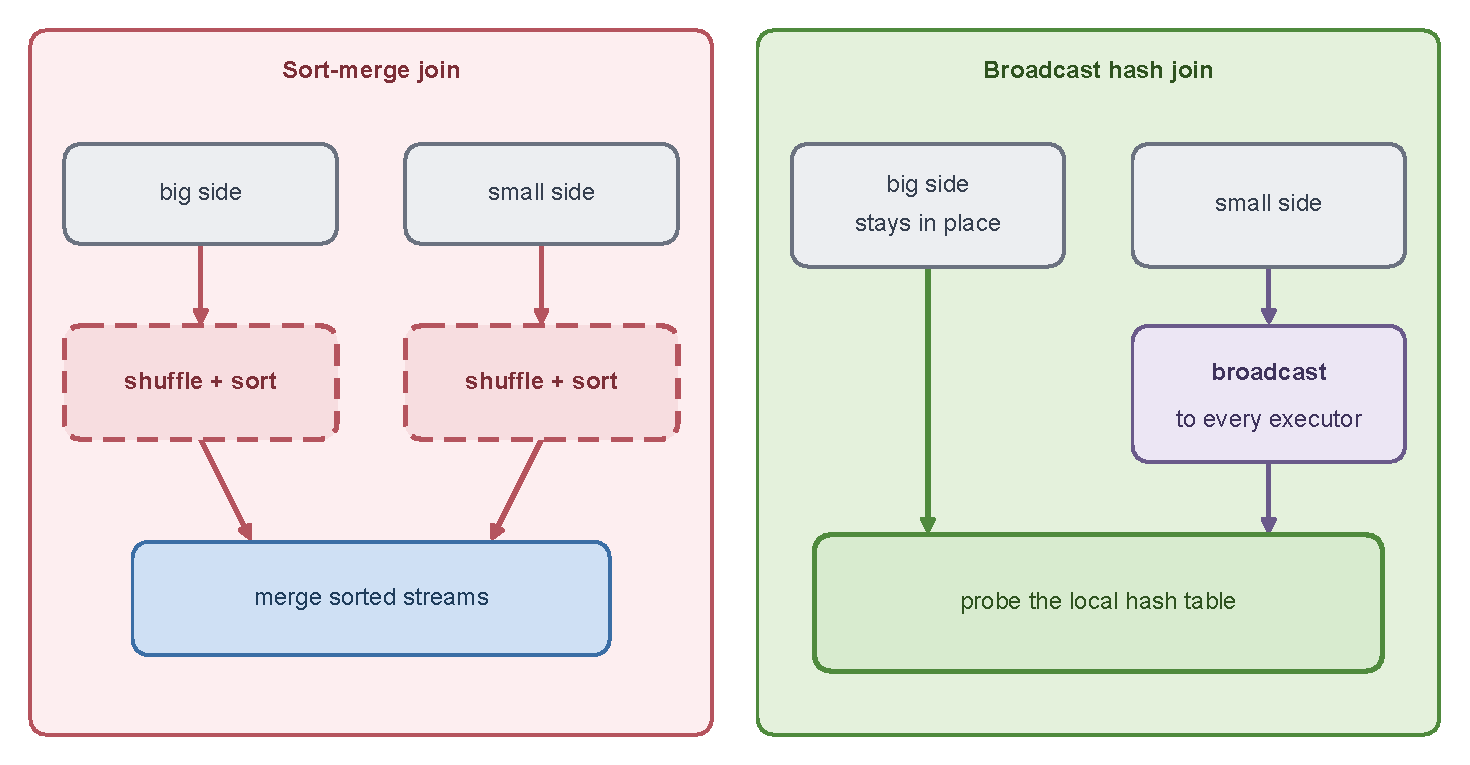
\includegraphics[width=\linewidth]{broadcast-vs-smj.pdf}
  \caption{The two cheapest-to-compare strategies side by side. A sort-merge join shuffles and sorts both sides before merging; a broadcast hash join leaves the big side in place and ships the small side to every executor.}
  \label{fig:broadcast-vs-smj}
\end{figure}

\section{Broadcast hash join}
\label{sec:joins-bhj}

If one side of a join is small enough, Spark skips shuffling the large side
entirely: it collects the small side to the driver, packages it once, and ships
a full copy to every executor (a \conf{BroadcastExchange}), where it is built
into an in-memory hash table keyed on the join column. Each task on the large
side then probes that local hash table row by row --- no shuffle, no sort, and
the large side is read exactly once, in place.

This is the cheapest strategy whenever it applies, which is exactly why the
planner tries it first. Two costs are easy to underestimate. First, the
\emph{driver} holds the whole broadcast table in memory while assembling it,
at roughly twice the table's serialized size; a broadcast large enough to hurt
the driver is a self-inflicted wound distinct from anything happening on the
executors. Second, the size used to decide broadcastability is the table's
\emph{on-disk} size, and a compressed columnar file routinely decodes to
several times that once it is rows in memory (\Cref{sec:mem-heap}) --- so a
``100~MB'' table can be genuinely 500~MB--1~GB once broadcast and decoded,
which is why the planning-time threshold is conservative by design. Spark also
enforces a hard ceiling (roughly 8~GB serialized, and a few hundred million
rows) past which a table cannot be broadcast at all, regardless of the
threshold.

Put numbers on it, from the lab (\Cref{sec:refenv-lab}). Filter
\texttt{dim\_product} to one category and 100\,000 rows remain. Spark's own
statistics for that side's shuffle read \texttt{3.8 MiB}; the broadcast relation
built from those same rows measured \texttt{20.0 MiB} in memory, more than five
times larger (\Cref{lst:aqe-broadcast-plan}). A threshold compared against the
first number is therefore a weak guard for the second, and the driver holds
roughly two copies of that relation while it collects the rows and builds the
payload to ship out. A dimension ten times larger inflates the same way, which
is why the comfortable-looking 10~MB threshold still leaves real headroom
before it threatens a driver's heap.

\section{Shuffle hash join}
\label{sec:joins-shj}

When neither side is small enough to broadcast but one side is still
meaningfully smaller than the other, Spark can shuffle both sides on the join
key and build an in-memory hash table from the smaller (build) side on each
executor, then probe it with the larger (probe) side --- without sorting
either. This is a \conf{ShuffledHashJoin}: two shuffles, like sort-merge, but
no \texttt{Sort} nodes, which makes it cheaper than sort-merge whenever the
build side reliably fits in memory per partition.

That condition is also its weakness: unlike sort-merge, a shuffled hash join
has no graceful way to spill an oversized build-side partition to disk. If a
single partition's build side is larger than expected --- most often because of
skew --- the task fails outright rather than slowing down. Spark's planner is
correspondingly conservative about choosing it: by default it prefers
sort-merge whenever both sides have sortable keys
(\conf{spark.sql.join.preferSortMergeJoin}\,=\,\texttt{true}), and only
considers a shuffled hash join when that preference is turned off and the
build side is estimated at at least three times smaller than the probe side.
Concretely: with the preference off, an estimated 500~MB \texttt{dim\_customer}
against a 2~GB \texttt{orders} slice qualifies (2~GB is $4\times$ larger), and
the plan shows \conf{ShuffledHashJoin} with no \texttt{Sort} node on either
input; the same 500~MB against only 1~GB of \texttt{orders} does not qualify
($2\times$, short of the $3\times$ bar), and the planner falls back to
sort-merge instead, adding a \texttt{Sort} node to each side of the plan that
was absent in the qualifying case.

\section{Sort-merge join}
\label{sec:joins-smj}

Sort-merge join is the default for two large, roughly comparable inputs, and it
is what the specimen query uses in \Cref{ch:catalyst}, because
\texttt{dim\_product} (about 170~MB) is far over the broadcast threshold: both
sides are shuffled on the join key, each partition is then sorted locally, and the join is
produced by walking both sorted streams together, advancing whichever key is
behind. It is the most expensive of the equi-join strategies --- two shuffles
and two sorts --- but it is also the most robust: a sort spills to disk cleanly
under memory pressure the way a hash table cannot, so it scales to inputs of any
size on either side.

\section{Broadcast nested loop join}
\label{sec:joins-bnlj}

An equi-join needs a hash or a sort; a join whose condition is not an equality
--- \texttt{ON o.order\_total > c.credit\_limit}, for instance --- needs neither, and
Spark falls back to comparing every row of one side against every row of the
other. If one side is small enough to broadcast, this is a
\conf{BroadcastNestedLoopJoin}: no shuffle, but $O(N \times M)$ comparisons
inside each task. If neither side is small enough to broadcast, Spark falls all
the way back to a \conf{CartesianProduct} (\Cref{sec:c-joins}), which is
rarely what you want on two large tables and is usually a sign that a join
condition is missing.

\begin{note}
A full outer join cannot use broadcast hash join, even with an explicit hint:
there is no way to detect an unmatched row on the broadcast side without
scanning it, which the strategy is built to avoid. A \texttt{FULL OUTER} join
falls back to sort-merge regardless of size.
\end{note}

\section{How the planner chooses}
\label{sec:joins-selection}

For an equi-join, the planner tries strategies in a fixed order, stopping at
the first one that applies (\Cref{fig:join-selection-flow}):

\begin{enumerate}
  \item an explicit join hint, if the query has one (\Cref{sec:joins-forcing});
  \item \textbf{broadcast hash join}, if either side's estimated size is at or
        below \conf{spark.sql.autoBroadcastJoinThreshold} (10~MB by default);
  \item \textbf{sort-merge join}, if \conf{spark.sql.join.preferSortMergeJoin}
        is \texttt{true} (the default) and the keys are sortable;
  \item \textbf{shuffled hash join}, if that preference is off and the build
        side is estimated at least $3\times$ smaller than the probe side and
        fits per-partition memory;
  \item \textbf{sort-merge join}, as the fallback for any remaining equi-join
        with sortable keys.
\end{enumerate}

\begin{figure}[htbp]
  \centering
  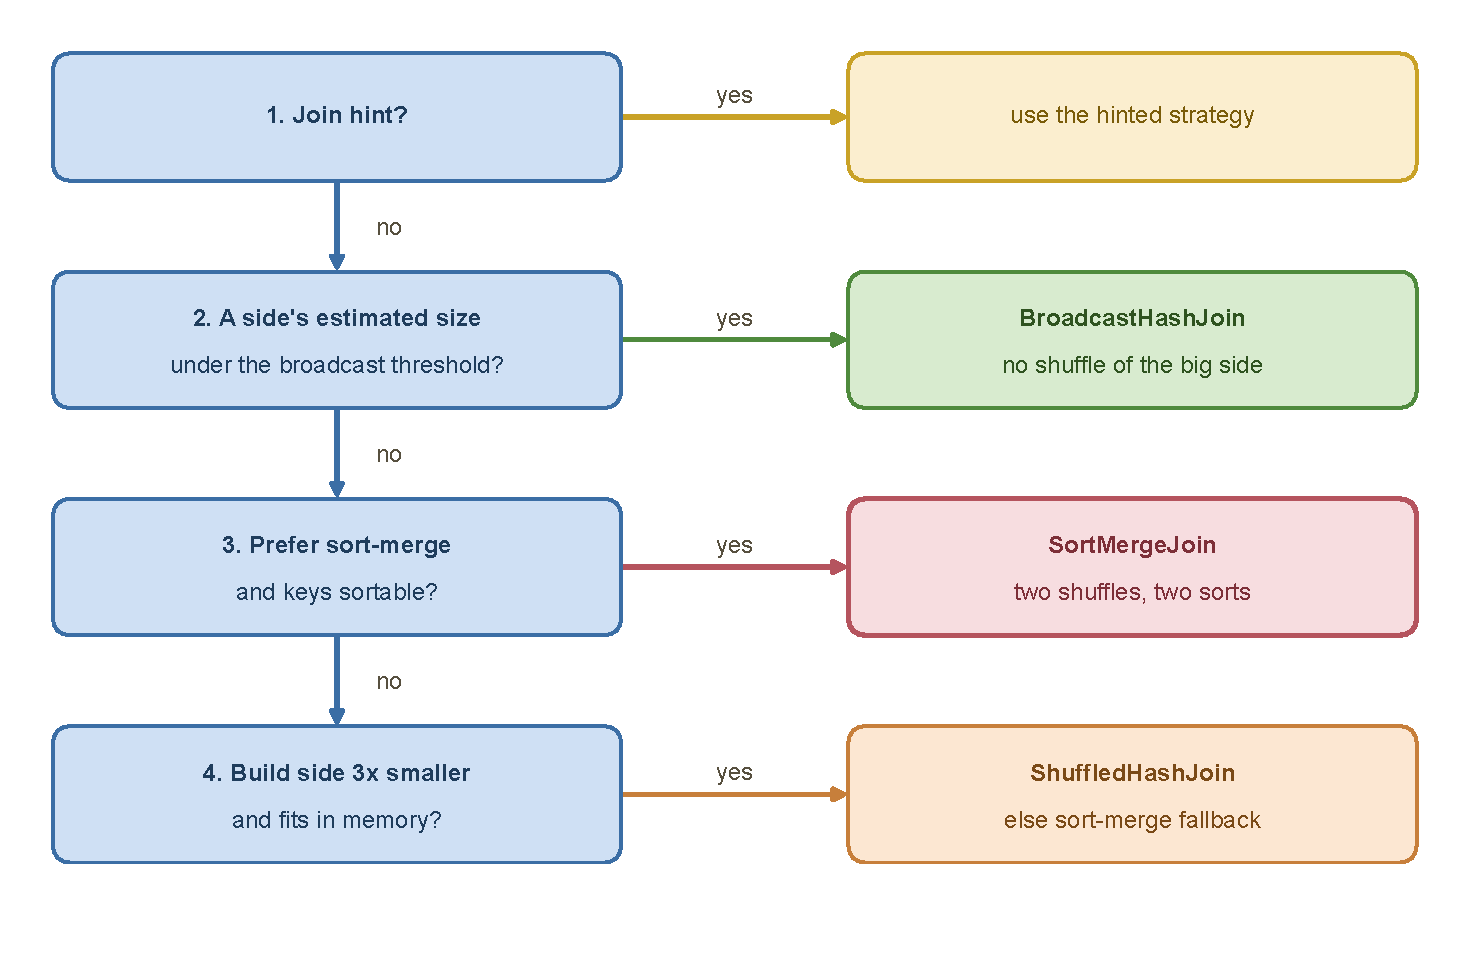
\includegraphics[width=\linewidth]{join-selection-flow.pdf}
  \caption{The planner stops at the first rule that applies. A hint wins outright; otherwise the estimated size decides, and sort-merge is the default for two large sides.}
  \label{fig:join-selection-flow}
\end{figure}

Every one of these decisions, except the explicit hint, is made from
\emph{estimated} sizes --- from the catalog if statistics exist, or from
on-disk file size if they do not (\Cref{sec:catalyst-analysis}). This is the
single most common way real joins go wrong: not a bug, but a plan built on a
wrong number.

Trace one query through the ordered list to see how the choice actually
falls out. For \texttt{orders JOIN dim\_customer}, with
\texttt{dim\_customer} estimated at 500~MB and no hint present: step~1 does
not apply (no hint); step~2 does not apply (500~MB is far past the 10~MB
threshold); step~3 \emph{does} apply --- \conf{preferSortMergeJoin} is
\texttt{true} by default and both join keys are plain strings, sortable ---
so the planner stops right there and emits a sort-merge join. Step~4 (the
shuffled-hash-join check) is never even evaluated, because the search stops
at the first rule that matches; a shuffled hash join only becomes reachable
at all if someone first turns \conf{preferSortMergeJoin} off, which is why
\Cref{sec:joins-shj} described it as the strategy the planner reaches for
last, not by default.

\section{What the strategies cost, measured}
\label{sec:joins-measured}

The lab forced each equi-join strategy with a hint on three dimensions of
different shape and joined each to the 30-million-row \texttt{orders} table, with
AQE off and automatic broadcast disabled so that only the hint decides
(\Cref{fig:join-strategy-times}). The plan operator was checked in every run: each
hint produced the operator it names.

\begin{figure}[htbp]
  \centering
  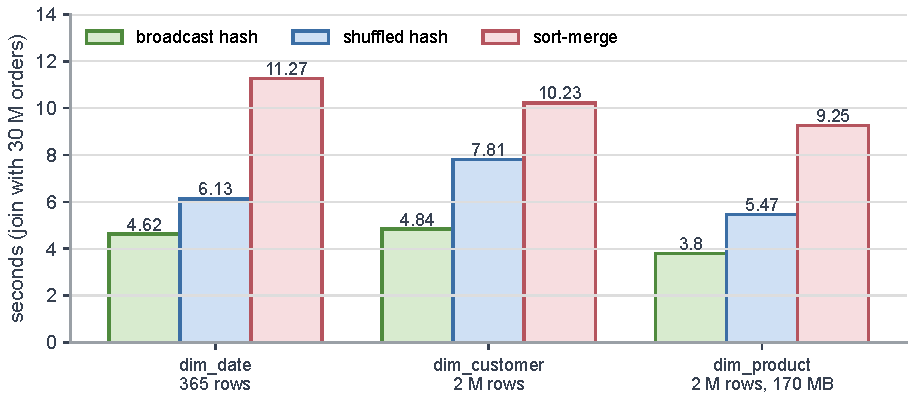
\includegraphics[width=\linewidth]{join-strategy-times.pdf}
  \caption{Seconds for the same join under each strategy. Broadcast was fastest on
  all three dimensions (3.8--4.8~s), shuffled hash in between (5.5--7.8~s) and
  sort-merge slowest (9.3--11.3~s). Each run has two exchanges for broadcast and
  three for the shuffled strategies.}
  \label{fig:join-strategy-times}
\end{figure}

Two readings. First, the ordering follows the work each strategy skips: broadcast
avoids shuffling the large side; shuffled hash shuffles both sides but builds a hash
table instead of sorting; sort-merge shuffles and sorts both. Second, broadcast won
even for the 2-million-row, 170~MB \texttt{dim\_product}, which the default
planner would \emph{not} broadcast (its estimate of 216~MB exceeds the 10~MB
threshold, \Cref{tab:dsv2-stats}): the threshold is a safety rail against driver
and executor memory, not the point where broadcast stops being faster. A
non-equi condition leaves two choices (\Cref{sec:joins-bnlj}); with a
\texttt{BROADCAST} hint the plan was a \conf{BroadcastNestedLoopJoin} (8.1~s for
200,000 rows against 365), and a \texttt{MERGE} hint on the non-equi condition was
ignored in favour of a \conf{CartesianProduct}.

\begin{warning}
A join hint names the \emph{alias} when the table is aliased. The first lab run wrote
\conf{BROADCAST(dim_date)} against \texttt{JOIN dim\_date d}: no error, no
warning, and a sort-merge join in every plan. If a hint seems ignored, read the
operator in \texttt{EXPLAIN} before concluding the optimizer overruled it.
\end{warning}

\section{Forcing a strategy}
\label{sec:joins-forcing}

When the estimate is wrong, a hint overrides it directly. The planner sees
\texttt{dim\_product} at its full 170~MB and will not broadcast it, but you know
the \texttt{category} filter leaves a few megabytes:

\begin{lstlisting}[language=SQL,caption={Forcing a broadcast of a filtered dimension},captionpos=b,label=lst:joins-hint]
SELECT /*+ BROADCAST(p) */ o.product_id, p.category
FROM orders o
JOIN (SELECT * FROM dim_product WHERE category = 'books') p
  ON o.product_id = p.product_id;
\end{lstlisting}

The hints, in priority order, are \texttt{BROADCAST} (or
\texttt{BROADCASTJOIN}/\texttt{MAPJOIN}), \texttt{SHUFFLE\_MERGE} (or
\texttt{MERGE}) for sort-merge, and \texttt{SHUFFLE\_HASH} for a shuffled hash
join. A hint is an instruction, not a suggestion: Spark will honor it even when
its own estimate disagrees, so a stale hint on a table that has since grown
past a sane broadcast size is a real production hazard, not a theoretical one.

The more durable fix is to give the planner real numbers instead of overriding
its guess:

\begin{lstlisting}[language=SQL,caption={Giving the CBO real statistics},captionpos=b]
ANALYZE TABLE db.dim_product COMPUTE STATISTICS FOR ALL COLUMNS;
\end{lstlisting}

Iceberg tables carry file-level size and row counts in their metadata for free,
so the planner's size estimate for an \emph{unfiltered} table is accurate;
\texttt{dim\_product}'s 170~MB is why the specimen shuffled it in
\Cref{ch:catalyst}. What Iceberg does not carry is the column-level statistics
the cost-based optimizer uses to estimate how much a \emph{filter} shrinks a
table, so a filtered scan is still estimated at full size. \texttt{ANALYZE}
supplies those statistics, and running it once after a table's data changes
materially is usually cheaper, and safer over time, than hard-coding a hint.
Whether it changes a particular join is something to measure, not assume.

\begin{tip}
Adaptive Query Execution catches many of these mistakes without any of the
above: it re-evaluates a join's strategy \emph{after} its inputs have shuffled,
against their real post-shuffle size, and promotes a sort-merge join to a
broadcast if the data turns out small enough (\Cref{ch:aqe}). Hints and
\texttt{ANALYZE} matter most for the joins AQE cannot rescue --- most often
because the small side is broadcastable only before a shuffle changes its
size, not after.
\end{tip}

\section{Storage-partitioned joins for bucketed Iceberg tables}
\label{sec:joins-spj}

Every strategy above pays the same structural cost sort-merge join pays most
visibly: two shuffles, one per side, every single time the query runs, even
though the join key never changes between runs. The next strategy exists to
avoid paying that cost at query time at all, by doing the equivalent work
once, up front, when the tables are written. Every strategy above assumes
the two sides arrive unaligned and have to be shuffled into agreement. If both tables are already \emph{bucketed} on the join
key with the same bucket count (\Cref{ch:iceberg-layout}), that assumption is
false: rows that must be compared are already co-located file by file, and
Spark can join corresponding buckets directly with no exchange on either
side --- a \emph{storage-partitioned join}. This turns the most expensive part
of a sort-merge join, the two shuffles, into work done once at write time
instead of on every query that joins the tables.

The condition is strict: both tables need the identical bucket transform and
bucket count on the join column, and Spark needs
\conf{spark.sql.sources.v2.bucketing.enabled} set to consider it at all. It is
a design decision made when the tables are created, not a query-time tuning
knob --- worth it specifically for a join pattern repeated often enough that
paying the shuffle cost once, at write time, beats paying it on every read.

\section{Summary}
\label{sec:joins-summary}

Four strategies, in the order the planner tries them: broadcast hash join
(cheapest, but bounded by the small side's real decoded size, not its file
size), sort-merge join (the robust default for two large sides), shuffled hash
join (cheaper than sort-merge when it applies, but unable to spill), and
broadcast nested loop or Cartesian for a non-equi condition. Every automatic
choice rests on a size estimate, and Iceberg tables commonly lack the
column statistics that estimate needs --- \texttt{ANALYZE TABLE} and join hints
exist specifically to correct that, and AQE corrects a real subset of it for
free at runtime. Bucketing both sides of a frequent join on the same key
removes the shuffle from the decision entirely.

\exercisehead
\begin{exercises}
\item Given four table sizes and the broadcast threshold, predict each join's
      strategy. Then change one config value and predict which join flips.
\item Run the specimen query and read the join strategy. Then raise
      \conf{spark.sql.autoBroadcastJoinThreshold} above \texttt{dim\_product}'s
      size and run it again. Predict the number of \texttt{Exchange} nodes
      before and after, and check against the plan.
\item Write a join with a non-equi condition on two tables, neither of which is
      small. Confirm in \texttt{EXPLAIN FORMATTED} that it becomes a
      \conf{CartesianProduct}, and rewrite it to avoid one.
\end{exercises}
